%\VignetteEngine{knitr::knitr}
%\VignetteDepends{RColorBrewer}
%\VignetteDepends{lattice}
%\VignetteDepends{nlme}
%\VignetteDepends{investr}
%\VignetteDepends{car}
%\VignetteDepends{lme4}
%\VignetteDepends{boot}
%\VignetteIndexEntry{Inverse estimation with linear mixed-effects models}

\documentclass[article]%{jss}

%% Packages
\usepackage{amsmath, bm, framed, booktabs}

%% Macros
\newcommand{\boot}{\ensuremath{^\star}}
\newcommand{\trans}{\ensuremath{^\top}}
\newcommand{\SE}{\operatorname{SE}}
\newcommand{\diag}{\operatorname{diag}}
\newcommand{\col}{\operatorname{col}}
\newcommand{\row}{\operatorname{row}}

%%%%%%%%%%%%%%%%%%%%%%%%%%%%%%
%% declarations for jss.cls %%%%%%%%%%%%%%%%%%%%%%%%%%%%%%%%%%%%%%%%%%
%%%%%%%%%%%%%%%%%%%%%%%%%%%%%%

%% almost as usual
\author{Brandon M. Greenwell\\Aptima, Inc \And
        Christine M. Schubert Kabban\\Air Force Institute of Technology}
\title{Inverse Estimation with Linear Mixed-Effects Models in \proglang{R}}

%% for pretty printing and a nice hypersummary also set:
\Plainauthor{Brandon M. Greenwell, Christine M. Schubert Kabban} %% comma-separated
\Plaintitle{Linear Calibration with Random Coefficients via the R Packages investr and lme4} %% without formatting
\Shorttitle{Linear Calibration with Random Coefficients} %% a short title (if necessary)

%% an abstract and keywords
\Abstract{
  Inverse estimation, more commonly known as calibration, is a classical and well-known problem in regression. In simple terms, it involves the use of an observed value of the response (or specified value of the mean response) to make inference on the corresponding unknown value of the explanatory variable.  In this paper, we describe how to calculate approximate calibration confidence intervals for the unknown value of the explanatory variable in random coefficient models using a well-known data set.
}
\Keywords{calibration, random coefficients, \pkg{investr}, \pkg{lme4}, \pkg{nlme}, \proglang{R}}
\Plainkeywords{calibration, random coefficients, investr, lme4, nlme, R} %% without formatting
%% at least one keyword must be supplied

%% publication information
%% NOTE: Typically, this can be left commented and will be filled out by the technical editor
%% \Volume{50}
%% \Issue{9}
%% \Month{June}
%% \Year{2012}
%% \Submitdate{2012-06-04}
%% \Acceptdate{2012-06-04}

%% The address of (at least) one author should be given
%% in the following format:
\Address{
  Brandon M. Greenwell\\
  Associate Research Engineer\\
  Aptima, Inc.\\
  3100 Presidential Drive, Suite 220\\
  Fairborn, OH 45324\\
  E-mail: \email{greenwell.brandon@gmail.com}\\
  URL: \url{https://github.com/w108bmg/investr}
%   URL: \url{http://www.aptima.com/about/aptima-team/brandon-greenwell}
}
%% It is also possible to add a telephone and fax number
%% before the e-mail in the following format:
%% Telephone: +43/512/507-7103
%% Fax: +43/512/507-2851

%% for those who use Sweave please include the following line (with % symbols):
%% need no \usepackage{Sweave.sty}

%% end of declarations %%%%%%%%%%%%%%%%%%%%%%%%%%%%%%%%%%%%%%%%%%%%%%%

\begin{document}

%% include your article here, just as usual
%% Note that you should use the \pkg{}, \proglang{} and \code{} commands.

%% Knitr stuff %%%%%%%%%%%%%%%%%%%%%%%%%%%%%%%%%%%%%%%%%%%%%%%%%%%%%%%%%%%%%%%%%




%%%%%%%%%%%%%%%%%%%%%%%%%%%%%%%%%%%%%%%%%%%%%%%%%%%%%%%%%%%%%%%%%%%%%%%%%%%%%%%%
%%%%%%%%%%%%%%%%%%%%%%%%%%%%%%%%%%%%%%%%%%%%%%%%%%%%%%%%%%%%%%%%%%%%%%%%%%%%%%%%
\section{Introduction}
%% Note: If there is markup in \(sub)section, then it has to be escape as above.

Consider an ordinary regression model $\mathcal{Y}_i = f\left( x_i; \bm{\beta} \right) + \epsilon_i$ $(i = 1, \dotsc, n)$, where $f$ is a known expectation function (called a \emph{calibration curve}) that is monotonic over the range of interest and $\epsilon_i \stackrel{iid}{\sim} \mathcal{N}\left( 0, \sigma^2 \right)$.  A common problem in regression is to predict a future response $\mathcal{Y}_0$ (or estimate the mean response $f_0$) for a known value of the explanatory variable $x_0$.  Often, however, there is a need to do the reverse; that is, given an observed value of the response $\mathcal{Y} = y_0$ (or a specified value of the mean response), estimate the unknown value of the explanatory variable $x_0$.  This is known as the \emph{calibration problem}, though it is often refered to more generally as inverse estimation.  A thorough overview of the calibration problem is given in \citet{osborne-statistical-1991}.  \citet{oman-calibration-1998} considers the case of a random intercept and slope model --- the goal of this paper is to show how easily this can be accomplished using a few packages from the \proglang{R} programming language.



%%%%%%%%%%%%%%%%%%%%%%%%%%%%%%%%%%%%%%%%%%%%%%%%%%%%%%%%%%%%%%%%%%%%%%%%%%%%%%%%
%%%%%%%%%%%%%%%%%%%%%%%%%%%%%%%%%%%%%%%%%%%%%%%%%%%%%%%%%%%%%%%%%%%%%%%%%%%%%%%%
\section{Linear Mixed-Effects Models}

Linear regression models with random coefficients can be represented in many different (but equivalent) forms.  One of the most common forms, attributed to \citet{laird-random-1982}, is
\begin{equation}
\label{eqn:lmm-laird-and-ware}
  \bm{\mathcal{Y}}_i = \bm{X}_i\bm{\beta} + \bm{Z}_i\bm{b}_i + \bm{\epsilon}_i, \quad i = 1, \dotsc, m,
\end{equation}
where
\begin{itemize}
  \item $\bm{\mathcal{Y}}_i$ is an $n_i \times 1$ response vector for the $i$-th subject/cluster/group;
  \item $\bm{X}_i$ is an $n_i \times p$ design matrix for the fixed effects;
  \item $\bm{Z}_i$ is an $n_i \times q$ design matrix for the random effects;
  \item $\bm{\beta}$ is a $p \times 1$ vector of fixed effects coefficients;
  \item $\bm{b}_i$ is a $q \times 1$ vector of random effects coefficients with mean zero and variance-covariance matrix $\bm{D}$;
  \item $\bm{D}$ is a $q \times q$ variance-covariance matrix for the random effects;
  \item $\bm{\epsilon}_i$ is an $n_i \times 1$ vector of random errors with mean zero and variance-covariance matrix $\sigma^2\bm{I}$.
\end{itemize}
Equation~\eqref{eqn:lmm-laird-and-ware} is known as a linear mixed-effects model (LMM).  The random effects and errors are often assumed to follow a normal distribution.  By stacking the data, the (normal) LMM can be written concisely as
\begin{equation}
\label{eqn:lmm-stacked}
    \bm{\mathcal{Y}} = \bm{X}\bm{\beta} + \bm{Z}\bm{b} + \bm{\epsilon}, \quad
      \begin{bmatrix}
        \bm{b} \\
        \bm{\epsilon}
      \end{bmatrix} \sim
      \mathcal{N}\left(\begin{bmatrix}
        \bm{0} \\
        \bm{0}
      \end{bmatrix}, \begin{bmatrix}
        \bm{D} & \bm{0} \\
        \bm{0} & \sigma^2\bm{I}
      \end{bmatrix}\right),
\end{equation}
where $\bm{\mathcal{Y}} = \col\left\{\bm{\mathcal{Y}}_i\right\}$, $\bm{X} = \col\left\{\bm{X}_i\right\}$, $\bm{Z} = \diag\left\{\bm{Z}_i\right\}$, $\bm{b} = \col\left\{\bm{b}_i\right\}$, and $\bm{\epsilon} = \col\left\{\bm{\epsilon}_i\right\}$ for $i = 1, \dotsc, m$.  Since $\COV\left[\bm{b}, \bm{\epsilon}\right] = \bm{0}$, it is assumed that the random vectors $\big\{ \bm{b}_i, \bm{\epsilon}_i \big\}_{i=1}^m$ are mutually independent.

The additional term $\bm{Z}\bm{b}$ in the model imposes a specific variance-covariance structure on the response vector $\bm{\mathcal{Y}}$:
\[
  \bm{\mathcal{Y}} \sim \mathcal{N}\left(\bm{X}\bm{\beta}, \bm{V}\right), \quad \bm{V} = \bm{Z}\bm{D}\bm{Z}\trans + \sigma^2\bm{I}.
\]
Thus, the fixed effects determine the mean of $\bm{\mathcal{Y}}$, while the random effects govern the variance-covariance structure of $\bm{\mathcal{Y}}$.  Different random effects structures impose different variance-covariance structures on the response resulting in a highly flexible framework for modelling \emph{grouped data}.

The random effects variance-covariance matrix $\bm{D}$ has at most $q(q+1)/2$ unique elements which we represent by the vector $\bm{\theta}$.  There are a number of methods available for estimating $\left( \bm{\beta}, \sigma^2, \bm{\theta} \right)$; see, for example, \citet[chap 6.]{mcculloch_generalized_2008} and \citet[chap. 2]{demidenko_mixed_2013}.  Most commonly, the fixed-effects $\bm{\beta}$ are estimated via the method of maximum likelihood (ML), while the variance components $\left(\sigma^2, \bm{\theta}\right)$ are estimated via restricted maximum likelihood (REML).  The ML estimator of $\bm{\beta}$, given by
\begin{equation*}
\widehat{\bm{\beta}} = \left( \bm{X}\trans \widehat{\bm{V}}^{-1} \bm{X} \right)\bm{X}\trans\bm{\mathcal{Y}},
\end{equation*}
depends on the estimated variance components through $\widehat{\bm{V}}$ which makes it difficult to capture the variability of $\widehat{\bm{\beta}}$ in small sample sizes (see \citet[pp. 165-167]{mcculloch_generalized_2008}).  The usual practice is to ignore the variability of the estimated variance components when making inference about the fixed effects; that is, treat $\widehat{\bm{V}}$ as the true (fixed) value of $\bm{V}$.  Modern computational procedures such as the parametric bootstrap and Markov chain Monte Carlo (MCMC) methods are two ways account for the variability of the estimated variance components.

%%%%%%%%%%%%%%%%%%%%%%%%%%%%%%%%%%%%%%%%
%%%%%%%%%%%%%%%%%%%%%%%%%%%%%%%%%%%%%%%%
\subsection{Bladder Volume Data}
For illustration, let us consider the bladder volume data which can be found in \citet[pg. 7]{brown-measurement-1993} and \citet{oman-calibration-1998}.  In Brown's words:
\begin{quotation}
\noindent``A series of 23 women patients attending a urodynamic clinic were recruited for the study. After successful voiding of the bladder, sterile water was introduced in additions of 1, 1.5, and then 2.5 cl increments up to a final cumulative total of 17.5 cl. At each volume a measure of height (\code{H}) in mm and depth (\code{D}) in mm of largest ultrasound bladder images were taken. The product \code{H} $\times$ \code{D} was taken as a measure of liquid volume.''
\end{quotation}
We took Brown's suggestion and transformed the data so that the relationship is approximately linear.  Spaghettiplots of both the original and transformed data are displayed in Figure~\ref{fig:spaghetti}.

\begin{knitrout}
\definecolor{shadecolor}{rgb}{0.969, 0.969, 0.969}\color{fgcolor}\begin{figure}[!htb]
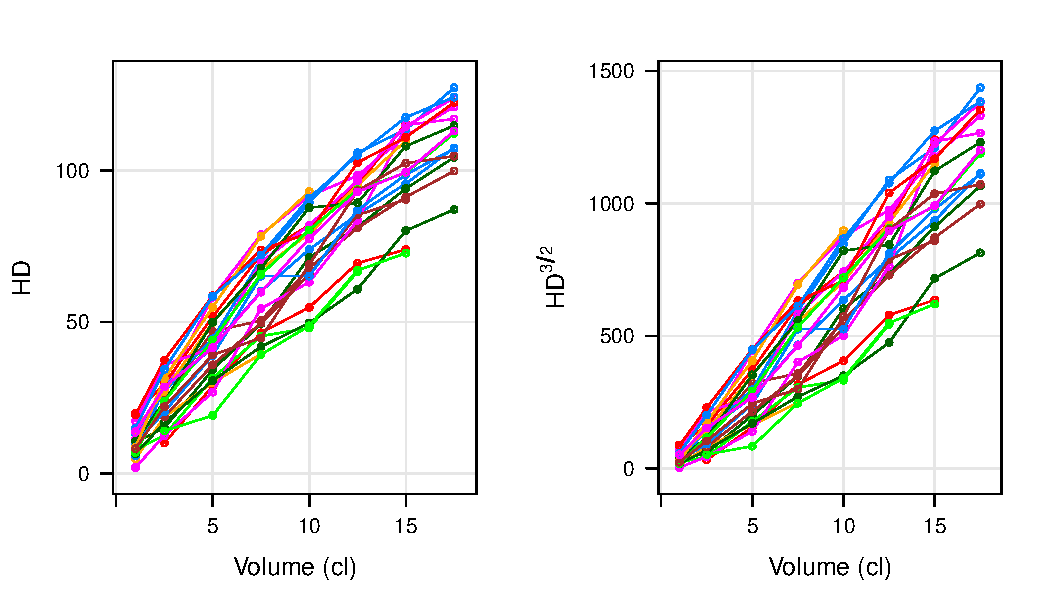
\includegraphics[width=\linewidth]{figure/spaghetti-1} \caption{Spaghettiplot of bladder volume data (lines connect measurements belonging to the same subject). \textit{Left}: Original data. \textit{Right}: Transformed data.}\label{fig:spaghetti}
\end{figure}


\end{knitrout}

A random intercept and slope model with uncorrelated random effects fits the transformed data well:
\begin{align*}
  \texttt{HD}^{3/2}_{ij} &= \left(\beta_0 + b_{0i}\right) + \left(\beta_1 + b_{1i}\right)\texttt{volume}_{ij} + \epsilon_{ij} \\
  b_{ki} &\sim \mathcal{N}\left(0, \theta_k^2\right), \quad k = 0, 1, \\
  \epsilon_{ij} &\sim \mathcal{N}\left(0, \sigma^2\right),
\end{align*}
where $\COV\left[b_{0i}, b_{1i}\right] = 0$.  To fit such a model in \proglang{R}, we can use the recommended \pkg{nlme} package \citep{pinheiro-nlme-2013} as follows:
\begin{knitrout}
\definecolor{shadecolor}{rgb}{0.969, 0.969, 0.969}\color{fgcolor}\begin{kframe}
\begin{alltt}
\hlkwd{library}\hlstd{(nlme)}  \hlcom{# nlme should already be installed}
\hlstd{(fit.nlme} \hlkwb{<-} \hlkwd{lme}\hlstd{(HD}\hlopt{^}\hlstd{(}\hlnum{3}\hlopt{/}\hlnum{2}\hlstd{)} \hlopt{~} \hlstd{volume,} \hlkwc{random} \hlstd{=} \hlkwd{list}\hlstd{(}\hlkwc{subject} \hlstd{=} \hlkwd{pdDiag}\hlstd{(}\hlopt{~}\hlstd{volume)),}
                 \hlkwc{data} \hlstd{= bladder))}
\end{alltt}
\begin{verbatim}
## Linear mixed-effects model fit by REML
##   Data: bladder 
##   Log-restricted-likelihood: -943
##   Fixed: HD^(3/2) ~ volume 
## (Intercept)      volume 
##       -53.8        69.1 
## 
## Random effects:
##  Formula: ~volume | subject
##  Structure: Diagonal
##         (Intercept) volume Residual
## StdDev:        39.6   14.3     53.7
## 
## Number of Observations: 166
## Number of Groups: 23
\end{verbatim}
\end{kframe}
\end{knitrout}
The \code{pdDiag} function forces a diagonal variance-covariance structure on the random effects; hence, a covariance of zero. The same model, but with an additional quadratic term, provides a useful fit to the original (untransformed) data:
\begin{align*}
  \texttt{HD}_{ij} &= \left(\beta_0 + b_{0i}\right) + \left(\beta_1 + b_{1i}\right)\texttt{volume}_{ij} + \beta_2\texttt{volume}_{ij}^2 + \epsilon_{ij} \\
  b_{ki} &\sim \mathcal{N}\left(0, \theta_k^2\right), \quad k = 0, 1, \\
  \epsilon_{ij} &\sim \mathcal{N}\left(0, \sigma^2\right).
\end{align*}
For an in-depth treatment on fitting LMMs using the \pkg{nlme} software, see \citet{pinheiro-mixed-2000}.



%%%%%%%%%%%%%%%%%%%%%%%%%%%%%%%%%%%%%%%%%%%%%%%%%%%%%%%%%%%%%%%%%%%%%%%%%%%%%%%%
%%%%%%%%%%%%%%%%%%%%%%%%%%%%%%%%%%%%%%%%%%%%%%%%%%%%%%%%%%%%%%%%%%%%%%%%%%%%%%%%
\section{Extending the Classical Methods of Calibration}
The standard methods of calibration, (i.e., the Wald-based and inversion confidence intervals) are easily extended to the case of random coefficients.  For convenience, let us write the linear random coefficient model as
\begin{equation*}
  \mathcal{Y}_{ij} = f\left(x_{ij}; \bm{\beta}\right) + R\left(x_{ij}; \bm{b}_i\right) + \epsilon_{ij},
\end{equation*}
where $f(\cdot)$ and $R(\cdot)$ are linear in $\bm{\beta}$ and $\bm{b}_i$, respectively.  For instance, the model for the transformed bladder data has $f\left(\texttt{volume}_{ij}; \bm{\beta}\right) = \beta_0 + \beta_1 \texttt{volume}_{ij}$ and $R\left(\texttt{volume}_{ij}; \bm{b}_i\right) = b_{0i} + b_{1i}\texttt{volume}_{ij}$ with $\VAR\left[R\left(\texttt{volume}_{ij}; \bm{b}_i\right)\right] = \theta_0^2 + \texttt{volume}_{ij}^2\theta_1^2$.

%%%%%%%%%%%%%%%%%%%%%%%%%%%%%%%%%%%%%%%%
%%%%%%%%%%%%%%%%%%%%%%%%%%%%%%%%%%%%%%%%
\subsection{Point Estimation}
Assume that, after the data are collected and a model is fitted, we obtain a new observation, denoted $\mathcal{Y}_0$, from the same population under study for which the value of the explanatory variable $x_0$ is unknown.  If we assume that the new observation belongs to a group not included in our analysis then estimating $x_0$ is rather straightforward.  By assumption, the new observation $\mathcal{Y}_0$ is distributed as a $\mathcal{N}\left\{f\left(x_0; \bm{\beta}\right), \sigma_0^2\right\}$ random variable with $\sigma_0^2 = \VAR\left[ R\left( x_0; \bm{b}_0 \right) \right ] + \sigma^2$.  A natural estimator for $x_0$ is then
\begin{equation}
\label{eqn:est}
  \widehat{x}_0 = f^{-1}\left(\mathcal{Y}_0; \widehat{\bm{\beta}}\right),
\end{equation}
where $\widehat{\bm{\beta}}$ is the ML estimator of $\bm{\beta}$.  We shall refer to Equation~\eqref{eqn:est} as the classical estimator.  Note that the point estimate $\widehat{x}_0$ does not involve any of the random effects; the random effects only contribute to the variance-covariance structure of the response.

%%%%%%%%%%%%%%%%%%%%%%%%%%%%%%%%%%%%%%%%
%%%%%%%%%%%%%%%%%%%%%%%%%%%%%%%%%%%%%%%%
\subsection{An Asymptotic Wald Interval}
\label{sec:wald}
An approximate $100(1-\alpha)\%$ Wald-type confidence interval for $x_0$ has the simple form
\begin{equation}
\label{eqn:wald}
  CI_{wald}\left(x_0\right)\left(x_0\right) = \left( \widehat{x}_0 -  \SE\left[\widehat{x}_0\right]\Phi\left(\alpha/2\right),  \widehat{x}_0 -  \SE\left[\widehat{x}_0\right]\Phi\left(1-\alpha/2\right) \right).
\end{equation}
There is no ``textbook'' formula for the standard error of $\widehat{x}_0$, instead, an estimate of this standard error is obtained using a first-order Taylor series approximation, or better yet, a bootstrap approximation.  For the Taylor series approximation, we need the variance-covariance matrix of $\left(\mathcal{Y}_0, \widehat{\bm{\beta}}\right)$,
\[
\Sigma = \begin{bmatrix}
           \VAR\left[\mathcal{Y}_0\right] & \bm{0} \\
           \bm{0} & \VAR\left[\widehat{\bm{\beta}}\right]
         \end{bmatrix} = \begin{bmatrix}
           \sigma_0^2 & \bm{0} \\
           \bm{0} & \left(\bm{X}\trans\bm{V}^{-1}\bm{X}\right)^{-1}
         \end{bmatrix}.
\]
Since $\mathcal{Y}_0$ is independent of $\bm{\mathcal{Y}}$, it is also independent of $\widehat{\bm{\beta}}$, hence the diagonal structure of $\Sigma$. Recall that our point estimate has the form $x = f^{-1}\left(y; \bm{\beta}\right)$. Let $f_1^{-1}\left(y; \bm{\beta}\right)$ and $f_2^{-1}\left(y; \bm{\beta}\right)$ denote the partial derivatives of $f^{-1}$ with respect to the parameters $y$ and $\bm{\beta}$, respectively. Our point estimator is given by $f^{-1}\left(\mathcal{Y}_0; \widehat{\bm{\beta}}\right)$, where $\mathcal{Y}_0$ is a new observation and $\widehat{\bm{\beta}}$ is the ML estimator of $\bm{\beta}$.  A first-order Taylor-series approximation for the variance of $\widehat{x}_0$ is given by
\begin{align}
  \VAR\left[\widehat{x}_0\right] &= \left[f_1^{-1}\left(\mathcal{Y}_0; \widehat{\bm{\beta}}\right)\right]^2\sigma_0^2 \nonumber \\
   &+ \left[f_2^{-1}\left(\mathcal{Y}_0; \widehat{\bm{\beta}}\right)\right]\trans\left(\bm{X}\trans\bm{V}^{-1}\bm{X}\right)^{-1}\left[f_2^{-1}\left(\mathcal{Y}_0; \widehat{\bm{\beta}}\right)\right].
\end{align}
To obtain $\SE\left[\widehat{x}_0\right] = \Big\{ \widehat{\VAR}\left[\widehat{x}_0\right] \Big\}^{1/2}$, we simply replace $\sigma_0^2$ and $\bm{V}$ with their respective estimates $\widehat{\sigma}_0^2$ and $\widehat{\bm{V}}$.

The Wald-based interval is simple to compute as long as we have an estimate for the standard error.  As we will discuss in Section~\ref{sec:implementation}, the \proglang{R} package \pkg{investr} \citep{investr-package} can be used to obtain the Wald-based interval \eqref{eqn:wald} using a Taylor series approximation of the standard error.  If a closed-form formula is available for $\widehat{x}_0$, then the \code{deltaMethod} function from the \pkg{car} package \citep{fox-car-2011} can also be used to obtain the Taylor series approximation of the standard error.  Alternatively, one can use a parametric bootstrap estimate of the standard error instead of relying on a Taylor series approximation --- see Section~\ref{sec:percentile}.  The bootstrap estimate may be more accurate in smaller sample sizes because, unlike the Taylor approximation estimate, it takes into account the variability of the estimated variance components.  The new \code{bootMer} function in the \pkg{lme4} package \citep{bates-lme4-2014} can be used for model-based parametric bootstrapping in mixed models.

%%%%%%%%%%%%%%%%%%%%%%%%%%%%%%%%%%%%%%%%
%%%%%%%%%%%%%%%%%%%%%%%%%%%%%%%%%%%%%%%%
\subsection{An Asymptotic Inversion Interval}
\label{sec:inversion}
In the case of the simple linear regression model with constant variance, an exact $100(1-\alpha)\%$ confidence interval for $x_0$ can be derived \citep{graybill-theory-1976}.  This can be generalized to an approximate method in the case of polynomial or nonlinear regression models with independent observations and constant variance (see \citet{seber-nonlinear-2003} and \citet{huet-statistical-2004}).  In a similar fashion, we can generalize the same results to an approximate method for random coefficient models.  Let $\widehat{f}_0 = f\left(x_0; \widehat{\bm{\beta}}\right)$ be the predicted mean at $x = x_0$.  A prediction interval for $\mathcal{Y}_0$ at $x_0$ with asymptotic coverage probability $100(1-\alpha)\%$ is
\begin{equation}
\label{eqn:asymptotic-pi}
  \mathcal{I}_\infty\left(x_0\right) = \widehat{f}_0 \pm z_{1-\alpha/2}\left\{ \widehat{\VAR}\left[\mathcal{Y}_0 - \widehat{f}_0\right] \right\}^{1/2}.
\end{equation}
If instead, $\mathcal{Y}_0$ is observed to be $y_0$ and $x_0$ is unknown, then an asymptotic $100(1-\alpha)\%$ confidence interval for the unknown $x_0$ can be obtained by inverting \eqref{eqn:asymptotic-pi}:
\begin{equation}
\label{eqn:inversion}
  CI_{inv}\left(x_0\right) = \left\{ x: z_{\alpha/2} \le \frac{\mathcal{Y}_0-f\left(x; \widehat{\bm{\beta}}\right)}{\left\{ \widehat{\VAR}\left[\mathcal{Y}_0 - f\left(x; \widehat{\bm{\beta}}\right)\right] \right\}^{1/2}} \le z_{1-\alpha/2} \right\}.
\end{equation}
This is known as the \emph{inversion interval} and typically cannot be written in closed-form; therefore, numerical techniques are required to find the lower and upper bounds.  Further, note that $CI_{inv}\left(x_0\right)$ is not symmetric about $\widehat{x}_0$ and will not necessarily result in a single finite interval.

Fortunately, the inversion interval \eqref{eqn:inversion} can be computed automatically using the \pkg{investr} package.  However, like the Wald-based interval \eqref{eqn:wald}, the inversion interval ignores the variability of the estimated variance components and will likely perform poorly in small sample sizes.  An alternative approach involving the parametric bootstrap will be discussed in Section~\ref{sec:parboot-inversion}.

Finally, the inversion interval uses a normal approximation.  While it is likely that a $t$~distribution with some finite degrees of freedom may be more accurate, it is difficult to find the appropriate degrees of freedom. \citet{oman-calibration-1998}, suggests a $t$~distribution with $N-1$ degrees of freedom ($N$ being the total sample size).



%%%%%%%%%%%%%%%%%%%%%%%%%%%%%%%%%%%%%%%%%%%%%%%%%%%%%%%%%%%%%%%%%%%%%%%%%%%%%%%%
\section{A Parametric Bootstrap Algorithm}
\label{sec:parboot}
The bootstrap \citep{efron-bootstrap-1979} is a general-purpose computer-based method for assessing accuracy of estimators and forming confidence intervals for parameters.  \citet{jones-bootstrapping-1999} proposed a nonparametric bootstrap algorithm for controlled calibration with independent observations.  However, since our application involves random coefficients (i.e., dependent observations), the nonparametric bootstrap does not easily apply, and instead, we adopt a ``fully parametric'' approach.  In a parametric bootstrap, bootstrap samples are generated from a fitted parametric model rather than sampling with replacement directly from the data.  Fortunately, parametric bootstrap confidence intervals are usually more accurate than nonparametric ones, however, by sampling from a fitted parametric family, we are implicitly assuming that we have the ``correct model''.

Let $\widehat{\sigma}_0^2$ be an estimate of the variance of the new observation $\mathcal{Y}_0$.  An algorithm for bootstrapping $\widehat{x}_0$ in an LMM is given in Figure~\ref{fig:parboot}.  Note that step 5. is crucial for calibration problems because we need to treat $y_0$ as a random quantity in the bootstrap simulation, otherwise the variability of $\widehat{x}_0$ will be underestimated; see, for example, \citet{jones-bootstrapping-1999} and \citet{greenwell-investr-2014}.
\begin{figure}[!htb]
\begin{framed}
\begin{enumerate}
  \item Fit a mixed model \eqref{eqn:lmm-stacked} to the data and obtain estimates $\widehat{\bm{\beta}}$, $\widehat{\bm{D}}$, and $\widehat{\sigma}^2$.
	\item Define $\bm{y}\boot = \bm{X}\widehat{\bm{\beta}} + \bm{Z}\bm{b}\boot + \bm{\epsilon}\boot$, where $\bm{b}\boot \sim \mathcal{N}_q\left(\bm{0}, \widehat{\bm{D}}\right)$ and $\bm{\epsilon}\boot \sim \mathcal{N}_N\left(\bm{0}, \widehat{\sigma}_\epsilon^2\bm{I}\right)$;
	\item Update the original model using $\bm{y}\boot$ as the response vector to obtain $\widehat{\bm{\beta}}\boot$ and $\widehat{\sigma}_0^{2\star}$;
	\item Generate $y_0\boot \sim \mathcal{N}\left(y_0, \widehat{\sigma}_0^{2\star}\right)$;
	\item Define $\widehat{x}_0\boot = f^{-1}\left(y_0\boot; \widehat{\bm{\beta}}\boot\right)$;
  \item Repeat steps (2)-(5) $R$ times.
\end{enumerate}
\end{framed}
\caption{Parametric bootstrap algorithm for linear calibration with random coefficients. \label{fig:parboot}}
\end{figure}

There are three main bootstrap confidence interval procedures: The percentile methods introduced in \citet{efron-bootstrap-1979}, the studentized bootstrap $t$ method introduced in \citet{efron-jackknife-1982}, and the double bootstrap method \citep{hall-bootstrap-1986}.  In this paper, we focus on the simple percentile interval and the studentized method.  For a good overview of all these confidence interval procedures, see \citet[chap. 5]{hinkley-bootstrap-1997} and \citet[chap. 11]{boos-essential-2013}.

%%%%%%%%%%%%%%%%%%%%%%%%%%%%%%%%%%%%%%%%
%%%%%%%%%%%%%%%%%%%%%%%%%%%%%%%%%%%%%%%%
\subsection{The percentile interval}
\label{sec:percentile}
The percentile method is the simplest and is given by the sample $\alpha/2$ and $1-\alpha/2$ quantiles of the bootstrap sample.  Let $\widehat{x}_{1*}, \dotsc, \widehat{x}_{R*}$ be a bootstrap sample obtained from the algorithm in Figure~\ref{fig:parboot}.  If $\widehat{F}_R$ is the empirical distribution function of the bootstrap sample, then an approximate $100(1-\alpha)\%$ confidence interval for $x_0$ is given by
\[
  \left( \widehat{F}_R^{-1}(\alpha/2), \widehat{F}_R^{-1}(1-\alpha/2) \right).
\]
The percentile interval is transformation respecting; thus, if we want a confidence interval for any one-to-one transformation $g\left(\widehat{x}_0\right)$, then we can just apply the transformation to the endpoints of the percentile interval for $\widehat{x}_0$.  The drawback is that the percentile interval is only \emph{first-order accurate} (see \citet[pp. 429-430]{boos-essential-2013}).  \citet{efron-better-1987} offered an improvement over the percentile interval called the \emph{bias-corrected and accelerated} ($BC_a$) interval that often obtains second-order accuracy and is transformation respecting.  However, the recommended \proglang{R} package \pkg{boot} \citep{canty-boot-2013} we will be relying on currently does not allow for $BC_a$ confidence intervals to be constructed from a parametric bootstrap.

%%%%%%%%%%%%%%%%%%%%%%%%%%%%%%%%%%%%%%%%
%%%%%%%%%%%%%%%%%%%%%%%%%%%%%%%%%%%%%%%%
\subsection{The bootstrap $t$ interval}
\label{sec:student}
A bootstrap $t$ interval for $x_0$ is essentially a bootstrap adjusted Wald-type interval.  The Wald interval for $x_0$ \eqref{eqn:wald} assumes that
\[
  Q_W = \frac{\widehat{x}_0 - x_0}{\SE\left[\widehat{x}_0\right]} \sim \mathcal{N}(0, 1).
\]
Rather than assuming that $Q_W$ is normal, the bootstrap $t$ method uses the bootstrap distribution of $Q_W\boot = \left(\widehat{x}_0\boot - \widehat{x}_0\right)/\SE\left[\widehat{x}_0\boot\right]$ to estimate the true distribution of $Q_W$.  If $\widehat{F}_{Q_W}$ is the empirical distribution function for a sample of $R$ bootstrap replicates of $Q_W$, then the bootstrap $t$  interval for $x_0$ is given by
\[
    CI_{wald}\left(x_0\right)\boot = \left( \widehat{x}_0 -  \SE\left[\widehat{x}_0\right]\widehat{F}_{Q_W}\left(\alpha/2\right),  \widehat{x}_0 -  \SE\left[\widehat{x}_0\right]\widehat{F}_{Q_W}\left(1-\alpha/2\right) \right).
\]
In order to implement this method, we need to calculate the standard error of each bootstrap replicate.  To do this, we can either use an additional (nested) bootstrap to estimate the standard error, or use a Taylor series approximation as discussed in Section~\ref{sec:wald}.  If time is  not a factor, then the nested bootstrap is preferred since bootstrap standard errors are usually more accurate than those based on a first-order Taylor series approximation \citep[pp. 478-480]{casella-statistical-2002}.  The benefits of using this interval over \eqref{eqn:wald} are that (a) it does not assume normality (hence, likely to be more accurate in smaller sample sizes) and (b) it is not symmetric about $\widehat{x}_0$; thus, more realistic when the response is nonlinear in $x$ (e.g., polynomials, etc.).

%%%%%%%%%%%%%%%%%%%%%%%%%%%%%%%%%%%%%%%%
%%%%%%%%%%%%%%%%%%%%%%%%%%%%%%%%%%%%%%%%
\subsection{Bootstrap adjusted inversion interval}
\label{sec:parboot-inversion}
\citet{huet-statistical-2004} suggests a bootstrap modification of the usual inversion interval in nonlinear regression models with dependent data.  In a similar fashion, we could use the parametric bootstrap to adjust the approximate inversion interval given in Equation~\eqref{eqn:inversion}.  The inversion interval assumes that the \emph{predictive pivot}
\[
  Q_I = \frac{\mathcal{Y}_0-f\left(x; \widehat{\bm{\beta}}\right)}{\left\{ \widehat{\VAR}\left[\mathcal{Y}_0 - f\left(x; \widehat{\bm{\beta}}\right)\right] \right\}^{1/2}} \sim \mathcal{N}(0, 1).
\]
A bootstrap modified inversion interval would then use the bootstrap distribution of
\[
  Q_I\boot = \frac{\mathcal{Y}_0\boot-f\left(\widehat{x}_0; \widehat{\bm{\beta}}\boot\right)}{\left\{ \widehat{\VAR}\left[\mathcal{Y}_0 - f\left(\widehat{x}_0; \widehat{\bm{\beta}}\boot\right)\right] \right\}^{1/2}},
\]
to estimate the true distribution of $Q_I$.  If $\widehat{F}_{Q_I}$ is the empirical distribution function for a sample of $R$ bootstrap replicates of $Q_I$, then the modified inversion interval for $x_0$ is given by
\[
    CI_{inv}\left(x_0\right)\boot = \left\{ x: \widehat{F}_{Q_I}\left(\alpha/2\right) \le Q_I \le \widehat{F}_{Q_I}\left(1-\alpha/2\right) \right\}.
\]
\vspace{25pt}

%%%%%%%%%%%%%%%%%%%%%%%%%%%%%%%%%%%%%%%%%%%%%%%%%%%%%%%%%%%%%%%%%%%%%%%%%%%%%%%%
\section[Implementation in R]{Implementation in \proglang{R}}
\label{sec:implementation}
Here, we discuss how to implement the previous procedures in the \proglang{R} programming languages.  We discuss two main packages: \pkg{investr} and \pkg{lme4}.  The \pkg{investr} package can be used for obtaining the Wald-based and inversion intervals.  This functionality is demonstrated over the next two sections.  The \pkg{lme4} package is a popular package for fitting linear, generalized linear, and nonlinear mixed models. Recently, however, the \pkg{lme4} package creators have added functionality for model-based parametric bootstrapping.  In Section~\ref{sec:lme4}, we demonstrate the potential of this new functionality by applying our parametric bootstrap algorithm to the bladder volume data discussed earlier.

%%%%%%%%%%%%%%%%%%%%%%%%%%%%%%%%%%%%%%%%
%%%%%%%%%%%%%%%%%%%%%%%%%%%%%%%%%%%%%%%%
\subsection[The investr package]{The \pkg{investr} package}
The \proglang{R} package \pkg{investr} facilitates calibration/inverse estimation with linear and nonlinear regression models.  The main function, \code{invest}, can be used for inverse estimation of $x_0$ given an observed response $y_0$.  More recently, the package has been updated to also handle objects of class \code{lme} from the \pkg{nlme} package.  Current functionality includes both the Wald-based and inversion methods outlined in Sections \ref{sec:wald}-\ref{sec:inversion}.  The main arguments for this function (as it applies to \code{lme} objects) are noted in Table~\ref{tab:invest} below.  The code for the package is hosted on GitHub at \url{https://github.com/w108bmg/investr}, but the latest stable release can be found on CRAN at \url{http://CRAN.R-project.org/package=investr}.

\begin{table}[!htb]
\begin{tabular}{lp{12cm}}
  \toprule
  Argument    & Description \\
  \midrule
  \code{object}        & An \proglang{R} object that inherits from class \code{lm}, \code{nls}, or \code{lme}. \\
  \code{y0}            & The value of the observed response. \\
  \code{interval}      & The type of interval required. Currently, only \code{"none"}, \code{"Wald"}, and \code{"inversion"} are supported. \\
  \code{level}         & A numeric scalar between 0 and 1 giving the confidence level for the interval to be calculated. The default is \code{0.95}. \\
  \code{lower}         & The lower endpoint of the interval to be searched. \\
  \code{upper} 				 & The upper endpoint of the interval to be searched. \\
  \code{q1}, \code{q2} & Optional quantiles to be used for constructing confidence intervals. \\
  \code{tol}           & The desired accuracy to be passed on to \code{uniroot}. \\
  \code{maxiter}       & The maximum number of iterations to be passed on to \code{uniroot}. \\
  \bottomrule
\end{tabular}
\caption{Main arguments for the \code{invest} function. \label{tab:invest}}
\end{table}

Returning to the bladder volume example, suppose we obtained an ultrasound measurement from a new patient for which $\texttt{HD}^{3/2} = 500$ (that's roughly 63 on the original scale).  What is the true volume of fluid ($x_0$) in the patients bladder?  We can estimate the true volume and form an approximate 95\% confidence interval using the methods discussed previously.  The point estimate is simply given by
\[
  \widehat{x}_0 = \frac{500 + 53.83164}{69.09491} = 8.0155 \text{ (cl)}.
\]
This estimate can be obtained in \proglang{R} as follows:
\begin{knitrout}
\definecolor{shadecolor}{rgb}{0.969, 0.969, 0.969}\color{fgcolor}\begin{kframe}
\begin{alltt}
\hlkwd{library}\hlstd{(investr)}
\hlstd{(x0.est} \hlkwb{<-} \hlkwd{invest}\hlstd{(fit.nlme,} \hlkwc{y0} \hlstd{=} \hlnum{500}\hlstd{,} \hlkwc{interval} \hlstd{=} \hlstr{"none"}\hlstd{))}
\end{alltt}
\begin{verbatim}
## [1] 8.02
\end{verbatim}
\end{kframe}
\end{knitrout}
The code used by \code{invest} to obtain this point estimate is basically
\begin{knitrout}
\definecolor{shadecolor}{rgb}{0.969, 0.969, 0.969}\color{fgcolor}\begin{kframe}
\begin{alltt}
\hlstd{fun} \hlkwb{<-} \hlkwa{function}\hlstd{(}\hlkwc{x}\hlstd{) \{}
  \hlkwd{predict}\hlstd{(fit.nlme,} \hlkwc{newdata} \hlstd{=} \hlkwd{list}\hlstd{(}\hlstr{"volume"} \hlstd{= x),} \hlkwc{level} \hlstd{=} \hlnum{0}\hlstd{)} \hlopt{-} \hlnum{500}
\hlstd{\}}
\hlkwd{uniroot}\hlstd{(fun,} \hlkwc{lower} \hlstd{=} \hlnum{1}\hlstd{,} \hlkwc{upper} \hlstd{=} \hlnum{17.5}\hlstd{,} \hlkwc{tol} \hlstd{=} \hlnum{1e-10}\hlstd{,} \hlkwc{maxiter} \hlstd{=} \hlnum{1000}\hlstd{)}\hlopt{$}\hlstd{root}
\end{alltt}
\begin{verbatim}
## [1] 8.02
\end{verbatim}
\end{kframe}
\end{knitrout}
In other words, \code{invest} relies on the function \code{uniroot} from the \pkg{stats} package to solve the equation $f\left(x; \widehat{\bm{\beta}}\right) - y_0 = 0$ numerically for $x$.  If the solution does not lie in the range of predictor values, then an error message will be displayed, as in
\begin{knitrout}
\definecolor{shadecolor}{rgb}{0.969, 0.969, 0.969}\color{fgcolor}\begin{kframe}
\begin{alltt}
\hlkwd{invest}\hlstd{(fit.nlme,} \hlkwc{y0} \hlstd{=} \hlnum{1500}\hlstd{)}
\end{alltt}


{\ttfamily\noindent\bfseries\color{errorcolor}{\#\# Error: Point estimate not found in the search interval (1, 17.5). Try tweaking the values of lower and upper.}}\end{kframe}
\end{knitrout}
The values for \code{lower}, \code{upper}, \code{tol}, and \code{maxiter} are controlled via the arguments of the same name listed in Table~\ref{tab:invest}.

When \code{interval = "Wald"}, an asymptotic $100(1-\alpha)\%$ confidence interval (where $\alpha$ is equal to \code{1 - level}) for $x_0$ is calculated according to Equation~\eqref{eqn:wald}:
\begin{knitrout}
\definecolor{shadecolor}{rgb}{0.969, 0.969, 0.969}\color{fgcolor}\begin{kframe}
\begin{alltt}
\hlkwd{invest}\hlstd{(fit.nlme,} \hlkwc{y0} \hlstd{=} \hlnum{500}\hlstd{,} \hlkwc{interval} \hlstd{=} \hlstr{"Wald"}\hlstd{)}
\end{alltt}
\begin{verbatim}
## estimate    lower    upper       se 
##     8.02     4.18    11.85     1.95
\end{verbatim}
\end{kframe}
\end{knitrout}
The standard error is computed using a First-order Taylor series approximation.   Similar to the code snippet shown below, \code{invest} calls the \pkg{stats} function \code{numericDeriv} to numerically evaluate the gradient of $\widehat{x}_0$ as a function of $y_0$ and $\widehat{\bm{\beta}}$.
\begin{knitrout}
\definecolor{shadecolor}{rgb}{0.969, 0.969, 0.969}\color{fgcolor}\begin{kframe}
\begin{alltt}
\hlstd{dmFun} \hlkwb{<-} \hlkwa{function}\hlstd{(}\hlkwc{params}\hlstd{) \{} \hlcom{# function of parameters whose gradient is required}
  \hlstd{fun} \hlkwb{<-} \hlkwa{function}\hlstd{(}\hlkwc{x}\hlstd{) \{}
    \hlstd{X} \hlkwb{<-} \hlkwd{model.matrix}\hlstd{(}\hlkwd{eval}\hlstd{(fit.nlme}\hlopt{$}\hlstd{call}\hlopt{$}\hlstd{fixed)[}\hlopt{-}\hlnum{2}\hlstd{],}
                      \hlkwc{data} \hlstd{=} \hlkwd{data.frame}\hlstd{(}\hlstr{"volume"} \hlstd{= x))}
    \hlstd{X} \hlopt \hlstd{params[}\hlopt{-}\hlkwd{length}\hlstd{(params)]} \hlopt{-} \hlstd{params[}\hlkwd{length}\hlstd{(params)]}
  \hlstd{\}}
  \hlkwd{uniroot}\hlstd{(fun,} \hlkwc{lower} \hlstd{=} \hlnum{1}\hlstd{,} \hlkwc{upper} \hlstd{=} \hlnum{17.5}\hlstd{,} \hlkwc{tol} \hlstd{=} \hlnum{1e-10}\hlstd{,}
          \hlkwc{maxiter} \hlstd{=} \hlnum{1000}\hlstd{)}\hlopt{$}\hlstd{root}
\hlstd{\}}
\hlstd{params} \hlkwb{<-} \hlkwd{c}\hlstd{(}\hlkwd{fixef}\hlstd{(fit.nlme),} \hlnum{500}\hlstd{)}
\hlstd{covmat} \hlkwb{<-} \hlkwd{diag}\hlstd{(}\hlnum{3}\hlstd{)}  \hlcom{# set up variance-covariance matrix}
\hlstd{covmat[}\hlnum{1}\hlopt{:}\hlnum{2}\hlstd{,} \hlnum{1}\hlopt{:}\hlnum{2}\hlstd{]} \hlkwb{<-} \hlkwd{vcov}\hlstd{(fit.nlme)}  \hlcom{# fixed effects var/cov matrix}
\hlstd{covmat[}\hlnum{3}\hlstd{,} \hlnum{3}\hlstd{]} \hlkwb{<-} \hlnum{17572.35}  \hlcom{# VAR[Y_0]}
\hlstd{gv} \hlkwb{<-} \hlkwd{attr}\hlstd{(}\hlkwd{numericDeriv}\hlstd{(}\hlkwd{quote}\hlstd{(}\hlkwd{dmFun}\hlstd{(params)),} \hlstr{"params"}\hlstd{),} \hlstr{"gradient"}\hlstd{)}
\hlstd{(se} \hlkwb{<-} \hlkwd{as.numeric}\hlstd{(}\hlkwd{sqrt}\hlstd{(gv} \hlopt \hlstd{covmat} \hlopt \hlkwd{t}\hlstd{(gv))))}
\end{alltt}
\begin{verbatim}
## [1] 1.95
\end{verbatim}
\end{kframe}
\end{knitrout}

Alternatively, one can use the very useful \code{deltaMethod} function from the \pkg{car} package to obtain \code{se}:
\begin{knitrout}
\definecolor{shadecolor}{rgb}{0.969, 0.969, 0.969}\color{fgcolor}\begin{kframe}
\begin{alltt}
\hlkwd{library}\hlstd{(car)}  \hlcom{# assuming package car is already installed}
\hlstd{params} \hlkwb{<-} \hlkwd{c}\hlstd{(}\hlkwd{fixef}\hlstd{(fit.nlme),} \hlnum{500}\hlstd{)}
\hlstd{covmat} \hlkwb{<-} \hlkwd{diag}\hlstd{(}\hlnum{3}\hlstd{)}  \hlcom{# set up var/cov matrix}
\hlstd{covmat[}\hlnum{1}\hlopt{:}\hlnum{2}\hlstd{,} \hlnum{1}\hlopt{:}\hlnum{2}\hlstd{]} \hlkwb{<-} \hlkwd{vcov}\hlstd{(fit.nlme)}  \hlcom{# fixed effects var/cov matrix}
\hlstd{covmat[}\hlnum{3}\hlstd{,} \hlnum{3}\hlstd{]} \hlkwb{<-}  \hlnum{17572.35}  \hlcom{# VAR[Y_0]}
\hlkwd{names}\hlstd{(params)} \hlkwb{<-} \hlkwd{c}\hlstd{(}\hlstr{"b0"}\hlstd{,} \hlstr{"b1"}\hlstd{,} \hlstr{"y0"}\hlstd{)}
\hlstd{(se} \hlkwb{<-} \hlkwd{deltaMethod}\hlstd{(params,} \hlkwc{g} \hlstd{=} \hlstr{"(y0 - b0)/b1"}\hlstd{,}  \hlkwc{vcov.} \hlstd{= covmat)}\hlopt{$}\hlstd{SE)}
\end{alltt}
\begin{verbatim}
## [1] 1.95
\end{verbatim}
\end{kframe}
\end{knitrout}
The only drawback here is that \code{deltaMethod} relies on the \pkg{stats} package symbolic differentiation function \code{D}; hence, $\widehat{x}_0 = f^{-1}\left(y_0; \widehat{\bm{\beta}}\right)$ has to be obtainable in closed-form.

To obtain the approximate inversion interval \eqref{eqn:inversion}, we specify \code{interval = "inversion"} (the default) as in the following:
\begin{knitrout}
\definecolor{shadecolor}{rgb}{0.969, 0.969, 0.969}\color{fgcolor}\begin{kframe}
\begin{alltt}
\hlkwd{invest}\hlstd{(fit.nlme,} \hlkwc{y0} \hlstd{=} \hlnum{500}\hlstd{,} \hlkwc{interval} \hlstd{=} \hlstr{"inversion"}\hlstd{)}
\end{alltt}
\begin{verbatim}
## estimate    lower    upper 
##     8.02     4.23    11.92
\end{verbatim}
\end{kframe}
\end{knitrout}
Essentially, \code{invest} finds the lower and upper inversion confidence limits \eqref{eqn:inversion} by solving the equations
\begin{equation*}
  Q_I - z_{\alpha/2} = 0 \quad \text{and} \quad Q_I - z_{1-\alpha/2} = 0
\end{equation*}
numerically for $x$ using the \proglang{R} function \code{uniroot}.  To use the quantiles from a $t$~distribution instead (see Section~\ref{sec:inversion}), we can supply them via the arguments \code{q1} and \code{q2}:
\begin{knitrout}
\definecolor{shadecolor}{rgb}{0.969, 0.969, 0.969}\color{fgcolor}\begin{kframe}
\begin{alltt}
\hlstd{N} \hlkwb{<-} \hlkwd{nrow}\hlstd{(bladder)}  \hlcom{# total sample size}
\hlstd{tvals} \hlkwb{<-} \hlkwd{qt}\hlstd{(}\hlkwd{c}\hlstd{(}\hlnum{0.025}\hlstd{,} \hlnum{0.975}\hlstd{),} \hlkwc{df} \hlstd{= N}\hlopt{-}\hlnum{1}\hlstd{)}  \hlcom{# quantiles from t distribution}
\hlkwd{invest}\hlstd{(fit.nlme,} \hlkwc{y0} \hlstd{=} \hlnum{500}\hlstd{,} \hlkwc{q1} \hlstd{= tvals[}\hlnum{1}\hlstd{],} \hlkwc{q2} \hlstd{= tvals[}\hlnum{2}\hlstd{])}
\end{alltt}
\begin{verbatim}
## estimate    lower    upper 
##     8.02     4.20    11.95
\end{verbatim}
\end{kframe}
\end{knitrout}
Being able to specify the arguments \code{q1} and \code{q2} will also be useful when implementing the bootstrap adjusted inversion interval described in Section~\ref{sec:parboot}

%%%%%%%%%%%%%%%%%%%%%%%%%%%%%%%%%%%%%%%%
%%%%%%%%%%%%%%%%%%%%%%%%%%%%%%%%%%%%%%%%
\subsection{Monte Carlo Study}
To assess the empirical performance of these confidence intervals, we carried out a small Monte Carlo study. The simulations described below were conducted in \proglang{R} using packages \pkg{plyr} \citep{wickham-plyr-2011}, \pkg{nlme}, and \pkg{lme4} \citep{bates-lme4-2014}.  The results are reported in Table~\ref{tab:simulation} and indicate that the Wald-based confidence interval \eqref{eqn:wald} and inversion confidence interval \eqref{eqn:inversion} have asymptotic coverage probability close to $100(1-\alpha)\%$.  This experiment also highlighted the fact that it is the number of subject $m$, not the sample size per subject $n$, that is more important for good asymptotic coverage.  The code used for the simulation is available upon request.

We consider the values 5, 10, 30, 50, and 100 for both the number of subjects $m$ and and the number of observations per subject $n$.  For each combination of sample sizes, we generated 1,000 data sets from a random intercept and slope model with parameters given by those listed in \code{summary(fit.nlme)}.  In other words, the fixed effects were $\bm{\beta} = \left(-53.83164, 69.09491\right)\trans$, the standard deviations for the (uncorrelated) random intercept and slope were 39.62499, and 14.28841, respectively.  The residual standard deviation was $\sigma = 53.71511$.  We chose $f\left(x_0; \bm{\beta}\right) = 500$ so that the true unknown is $x_0 = 8.0155$.  The standard deviation of the coverage estimates is approximately $\sqrt{0.95\left(1-0.95\right)/1000} = 0.001$.  A trellis plot of the results is given in Figure~\ref{fig:simulation}.  The coverage estimates are plotted against the number of subjects $m$ and paneled by number of observations per subject $n$.
\begin{table}[!htb]
\centering
\begin{tabular}{llccccc}
  \toprule
  %\rule{0pt}{4ex}
  $m$  & Method    & \hspace{8pt}$n = 5$\hspace{8pt} & \hspace{8pt}$n = 10$\hspace{8pt} & \hspace{8pt}$n = 30$\hspace{8pt} & \hspace{8pt}$n = 50$\hspace{8pt} & \hspace{8pt}$n = 100$ \hspace{8pt} \\
  \hline
  %\rule{0pt}{4ex}
  5    & Wald      & 0.89    & 0.89     & 0.89     & 0.87     & 0.89      \\
       & Inversion & 0.89    & 0.90     & 0.89     & 0.88     & 0.90      \\ \hline
  10   & Wald      & 0.92    & 0.92     & 0.94     & 0.93     & 0.93      \\
       & Inversion & 0.92    & 0.92     & 0.94     & 0.94     & 0.93      \\ \hline
  30   & Wald      & 0.95    & 0.95     & 0.95     & 0.94     & 0.95      \\
       & Inversion & 0.94    & 0.94     & 0.94     & 0.94     & 0.95      \\ \hline
  50   & Wald      & 0.95    & 0.96     & 0.95     & 0.94     & 0.94      \\
       & Inversion & 0.94    & 0.95     & 0.95     & 0.94     & 0.94      \\ \hline
  100  & Wald      & 0.95    & 0.95     & 0.95     & 0.94     & 0.94      \\
       & Inversion & 0.95    & 0.95     & 0.95     & 0.94     & 0.95      \\
  \bottomrule
\end{tabular}
\caption{Coverage probability of 95\% confidence intervals for simulated bladder data. \label{tab:simulation}}
\end{table}%\vskip18pt

\begin{knitrout}
\definecolor{shadecolor}{rgb}{0.969, 0.969, 0.969}\color{fgcolor}\begin{figure}[!htb]
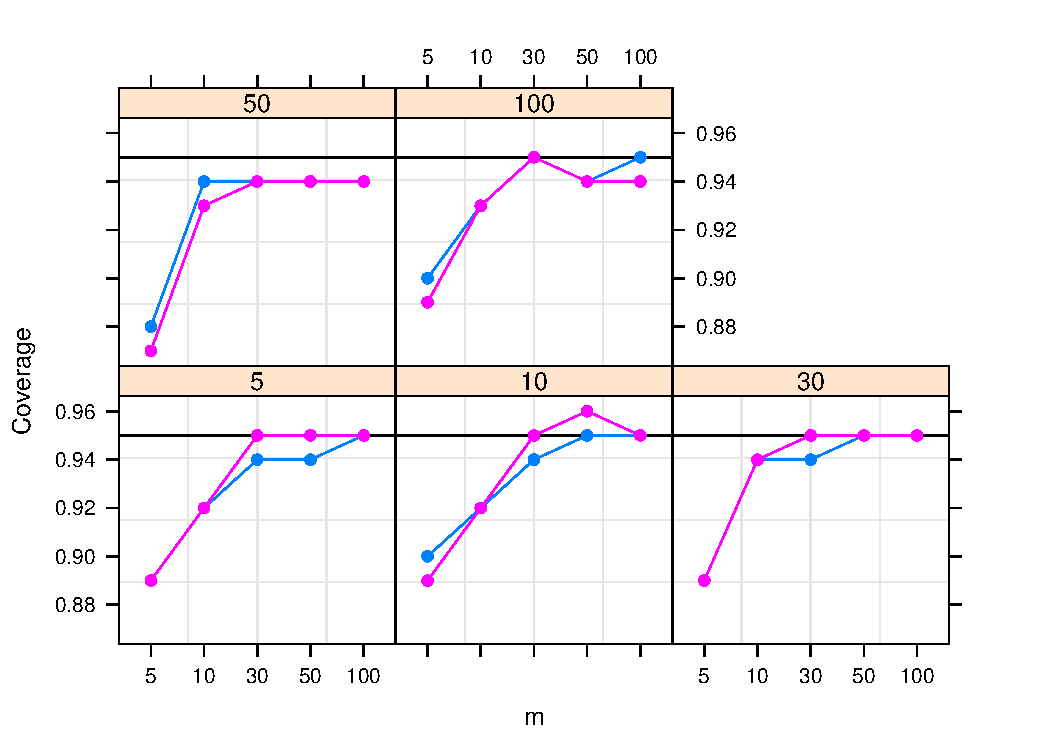
\includegraphics[width=\maxwidth]{figure/simulation-1} \caption[Coverage probability of 95\% confidence intervals for simulated bladder data]{Coverage probability of 95\% confidence intervals for simulated bladder data. The coverage estimates based on the inversion method are colored blue.}\label{fig:simulation}
\end{figure}


\end{knitrout}

%%%%%%%%%%%%%%%%%%%%%%%%%%%%%%%%%%%%%%%%
%%%%%%%%%%%%%%%%%%%%%%%%%%%%%%%%%%%%%%%%
\subsection[Using the lme4 package]{Using the \pkg{lme4} package}
\label{sec:lme4}
Implementation of the parametric bootstrap algorithm in Figure~\ref{fig:parboot} is relatively straight forward using the new \code{bootMer} function from the well-known \proglang{R} package \pkg{lme4} \citep{bates-lme4-2014} in conjunction with the \pkg{boot} package.

Since we will be using the \pkg{lme4} package, we need to refit the model using the \code{lmer} function:
\begin{knitrout}
\definecolor{shadecolor}{rgb}{0.969, 0.969, 0.969}\color{fgcolor}\begin{kframe}
\begin{alltt}
\hlkwd{library}\hlstd{(lme4)}  \hlcom{# assuming lme4 is already installed}
\hlstd{fit.lme4} \hlkwb{<-} \hlkwd{lmer}\hlstd{(HD2} \hlopt{~} \hlstd{volume} \hlopt{+} \hlstd{(}\hlnum{0}\hlopt{+}\hlnum{1}\hlopt{|}\hlstd{subject)} \hlopt{+} \hlstd{(}\hlnum{0}\hlopt{+}\hlstd{volume}\hlopt{|}\hlstd{subject),}
                 \hlkwc{data} \hlstd{= bladder)}
\end{alltt}
\end{kframe}
\end{knitrout}
Theoretically, the parameter estimates from this model should be the same as those from \code{fit.nlme}; however, there are likely to be small numerical differences between the two.  For this reason, let us re-estimate $\widehat{x}_0$ using \code{fit.lme4}.  Since \code{invest} does not work on objects of class \code{lmer}, we have to do things manually:
\begin{knitrout}
\definecolor{shadecolor}{rgb}{0.969, 0.969, 0.969}\color{fgcolor}\begin{kframe}
\begin{alltt}
\hlstd{fe} \hlkwb{<-} \hlkwd{unname}\hlstd{(}\hlkwd{fixef}\hlstd{(fit.lme4))}  \hlcom{# fixed effects without dimnames attribute}
\hlstd{(x0.est} \hlkwb{<-} \hlstd{(}\hlnum{500} \hlopt{-} \hlstd{fe[}\hlnum{1}\hlstd{])} \hlopt{/} \hlstd{fe[}\hlnum{2}\hlstd{])}
\end{alltt}
\begin{verbatim}
## [1] 8.02
\end{verbatim}
\end{kframe}
\end{knitrout}
Also, for convenience, we define the following function which estimates $\VAR\left[\mathcal{Y}|x\right] = \sigma_0^2 + x^2\sigma_1^2 + \sigma^2$ for a given value of $x$:
\begin{knitrout}
\definecolor{shadecolor}{rgb}{0.969, 0.969, 0.969}\color{fgcolor}\begin{kframe}
\begin{alltt}
\hlstd{var.y} \hlkwb{<-} \hlkwa{function}\hlstd{(}\hlkwc{object}\hlstd{,} \hlkwc{x}\hlstd{) \{}
  \hlstd{vc} \hlkwb{<-} \hlkwd{as.data.frame}\hlstd{(lme4}\hlopt{::}\hlkwd{VarCorr}\hlstd{(object))}\hlopt{$}\hlstd{vcov}
  \hlstd{vc[}\hlnum{1}\hlstd{]} \hlopt{+} \hlstd{vc[}\hlnum{2}\hlstd{]}\hlopt{*}\hlstd{x}\hlopt{^}\hlnum{2} \hlopt{+} \hlstd{vc[}\hlnum{3}\hlstd{]}
\hlstd{\}}
\end{alltt}
\end{kframe}
\end{knitrout}
For example, to estimate $\sigma_0^2 = \widehat{\VAR}\left[\mathcal{Y}_0\right]$, we have \code{var.y(fit.lme4, x = x0.est)}, which gives \ensuremath{1.757\times 10^{4}}, the same value used in the previous section.

Although we could easily compute all the bootstrap intervals previously discussed in one call to \code{bootMer} and \code{boot.ci}, we will discuss and compute each interval separately.

The following snippet of code generates $R = 9999$ bootstrap replicates of $\widehat{x}_0$, $Q_W$, and $Q_I$ according to the algorithm in Figure~\ref{fig:parboot}:
\begin{knitrout}
\definecolor{shadecolor}{rgb}{0.969, 0.969, 0.969}\color{fgcolor}\begin{kframe}
\begin{alltt}
\hlstd{boot.fun} \hlkwb{<-} \hlkwa{function}\hlstd{(}\hlkwc{.}\hlstd{) \{}  \hlcom{# bootstrap function}

  \hlcom{## Point estimate}
  \hlstd{var.y0.boot} \hlkwb{<-} \hlkwd{var.y}\hlstd{(.,} \hlkwc{x} \hlstd{= x0.est)}  \hlcom{# VAR[Y0]}
  \hlstd{fe.boot} \hlkwb{<-} \hlkwd{unname}\hlstd{(}\hlkwd{fixef}\hlstd{(.))}  \hlcom{# fixed effects}
  \hlkwa{if} \hlstd{(}\hlkwd{all}\hlstd{(}\hlkwd{getME}\hlstd{(.,} \hlstr{"y"}\hlstd{)} \hlopt{==} \hlstd{bladder}\hlopt{$}\hlstd{HD2)) \{}
    \hlstd{y0.boot} \hlkwb{<-} \hlnum{500}
  \hlstd{\}} \hlkwa{else} \hlstd{\{}
    \hlstd{y0.boot} \hlkwb{<-} \hlkwd{rnorm}\hlstd{(}\hlnum{1}\hlstd{,} \hlnum{500}\hlstd{,} \hlkwd{sqrt}\hlstd{(var.y0.boot))}
  \hlstd{\}}
  \hlstd{x0.boot} \hlkwb{<-} \hlstd{(y0.boot} \hlopt{-} \hlstd{fe.boot[}\hlnum{1}\hlstd{])}\hlopt{/}\hlstd{fe.boot[}\hlnum{2}\hlstd{]}

  \hlcom{## Approximate variance}
  \hlstd{covmat} \hlkwb{<-} \hlkwd{diag}\hlstd{(}\hlnum{3}\hlstd{)}
  \hlstd{covmat[}\hlnum{1}\hlopt{:}\hlnum{2}\hlstd{,} \hlnum{1}\hlopt{:}\hlnum{2}\hlstd{]} \hlkwb{<-} \hlkwd{as.matrix}\hlstd{(}\hlkwd{vcov}\hlstd{(.))}
  \hlstd{covmat[}\hlnum{3}\hlstd{,} \hlnum{3}\hlstd{]} \hlkwb{<-}  \hlstd{var.y0.boot}
  \hlstd{params} \hlkwb{<-} \hlkwd{c}\hlstd{(}\hlstr{"b0"} \hlstd{= fe.boot[}\hlnum{1}\hlstd{],} \hlstr{"b1"} \hlstd{= fe.boot[}\hlnum{2}\hlstd{],} \hlstr{"y0"} \hlstd{= y0.boot)}
  \hlstd{dm} \hlkwb{<-} \hlkwd{deltaMethod}\hlstd{(params,} \hlkwc{g} \hlstd{=} \hlstr{"(y0 - b0)/b1"}\hlstd{,}  \hlkwc{vcov.} \hlstd{= covmat)}
  \hlstd{var.x0.boot} \hlkwb{<-} \hlstd{dm}\hlopt{$}\hlstd{SE}\hlopt{^}\hlnum{2}

  \hlcom{## Approximate predictive pivot}
  \hlstd{mu0.boot} \hlkwb{<-}  \hlkwd{as.numeric}\hlstd{(}\hlkwd{crossprod}\hlstd{(fe.boot,} \hlkwd{c}\hlstd{(}\hlnum{1}\hlstd{, x0.est)))}
  \hlstd{var.mu0.boot} \hlkwb{<-} \hlkwd{t}\hlstd{(}\hlkwd{c}\hlstd{(}\hlnum{1}\hlstd{, x0.est))} \hlopt \hlkwd{as.matrix}\hlstd{(}\hlkwd{vcov}\hlstd{(.))} \hlopt \hlkwd{c}\hlstd{(}\hlnum{1}\hlstd{, x0.est)}
  \hlstd{QI.boot} \hlkwb{<-} \hlstd{(y0.boot} \hlopt{-} \hlstd{mu0.boot)}\hlopt{/}\hlkwd{sqrt}\hlstd{(var.y0.boot} \hlopt{+} \hlstd{var.mu0.boot)}

  \hlkwd{c}\hlstd{(x0.boot, var.x0.boot, QI.boot)}

\hlstd{\}}
\hlstd{pb} \hlkwb{<-} \hlkwd{bootMer}\hlstd{(fit.lme4, boot.fun,} \hlkwc{nsim} \hlstd{=} \hlnum{9999}\hlstd{,} \hlkwc{seed} \hlstd{=} \hlnum{105}\hlstd{)}  \hlcom{# run simulation}
\end{alltt}
\end{kframe}
\end{knitrout}
The \code{bootMer} function returns an object of class \code{boot} which can then be processed via the \pkg{boot} package to obtain the various bootstrap confidence intervals discussed earlier.  A basic summary of \code{pb} is given by
\begin{knitrout}
\definecolor{shadecolor}{rgb}{0.969, 0.969, 0.969}\color{fgcolor}\begin{kframe}
\begin{alltt}
\hlkwd{library}\hlstd{(boot)}  \hlcom{# load boot package}
\hlkwd{summary}\hlstd{(pb)}
\end{alltt}
\begin{verbatim}
##      R original bootBias bootSE bootMed
## 1 9999     8.02 -0.00219   1.97  8.0186
## 2 9999     3.82  0.05243   1.02  3.7702
## 3 9999     0.00 -0.00810   1.00  0.0016
\end{verbatim}
\end{kframe}
\end{knitrout}











